\section{Decay-time fit to $\Bs\to\Ds\pion\pion\pion$ and $\Bs\to\Ds\kaon\pion\pion$ candidates}
\label{sec:timeFit}

The sFit technique~\cite{Pivk:2004ty} is used to statistically subtract the background from the $\Bs\to\Ds\pion\pion\pion$ and $\Bs\to\Ds\kaon\pion\pion$ data samples. 
During the fit procedure, $\Gs$ and $\DGs$ are fixed to the corresponding HFLAV~\cite{HFAG} world average.
The $\Bs$ production asymmetry $A_{p}$, defined as the relative difference in the production cross sections $\frac{\sigma(\Bsb) - \sigma(\Bs)}{\sigma(\Bsb) + \sigma(\Bs)}$, contributes with a factor $(1 \pm A_{p})$ to the signal PDF,
where the sign depends on the flavour of the b meson. 
For data recorded during Run I, $A_{p}$ is taken from~\cite{Aaij:2017mso}.
The PDFs used for the fits to the $\Bs\to\Ds\pion\pion\pion$ and $\Bs\to\Ds\kaon\pion\pion$ candidates are convolved with a Gaussian function representing the per-candidate decay-time resolution 
and multiplied by the decay-time acceptance described in Sections \ref{sec:Resolution} and \ref{sec:Acceptance}, respectively.\newline

Since the decay $\Bs\to\Ds\pion\pion\pion$ is flavour specific, the \CP coefficients defined in Equation xXx can be fixed to $C=1$ and $D_{f} = D_{\bar{f}} = S_{f} = S_{\bar{f}} = 0$. 
In the fit, the calibration parameters for the OS and SS taging algorithms, the $\Bs$ production asymmetry for Run II data, as well as the $\Bs$ oscillation frequency $\dms$, are measured.  
The fit to the decay-time distribution is shown in Figure \ref{fig:tFitNorm} and the measured observables are summarized in Table \ref{tab:normFitResults}. 

\begin{table}[h]
\centering
\footnotesize
\caption{\small Parameters determined from a fit to the $B_s \to D_s \pi \pi\pi$ decay-time distribution. The uncertainties are statistical and systematic, respectively.}
%\resizebox{\linewidth}{!}{
        \renewcommand{\arraystretch}{1.25}
        \begin{tabular}{l c c c c } 
\hline
\hline
\multicolumn{1}{c}{Decay Channel} & \multicolumn{2}{c}{$A_{b \to c}$} & \multicolumn{2}{c}{$A_{b \to u}$}  \\ 
 & \multicolumn{1}{c}{$\vert a_i \vert$}  & \multicolumn{1}{c}{$arg(a_i) [\degrees]$}  & \multicolumn{1}{c}{$\vert a_i \vert$} & \multicolumn{1}{c}{$arg(a_i) [\degrees]$} \\ 
\hline
 $B_s \to D_s \, ( K_1(1270) \to K \, \rho(770) ) $ &  1.0 & 0.0 & 1.0 & 0.0  \\ 
$\phantom{B_s \to D_s \, (} K_1(1270) \to K^{*}(892) \, \pi \phantom{)} $ & 0.76 $\pm$ 0.11 $\pm$ 0.16 & 60.9 $\pm$ 9.6 $\pm$ 14.0 & &   \\ 
$\phantom{B_s \to D_s \, (} K_1(1270) \to K^{*}_{0}(1430) \, \pi \phantom{)} $ & 0.68 $\pm$ 0.06 $\pm$ 0.34 & 116.5 $\pm$ 5.1 $\pm$ 43.5 & &   \\ 
$B_s \to D_s \, ( K_1(1400) \to K^{*}(892) \, \pi ) $ & 2.53 $\pm$ 0.27 $\pm$ 0.57 & 12.9 $\pm$ 7.4 $\pm$ 8.0 & 0.67 $\pm$ 0.20 $\pm$ 0.51 & -76.3 $\pm$ 16.9 $\pm$ 22.8 \\ 
$B_s \to D_s \, ( K^{*}(1410) \to K^{*}(892) \, \pi ) $ & 1.28 $\pm$ 0.12 $\pm$ 0.24 & 54.9 $\pm$ 5.6 $\pm$ 9.8 &  &  \\ 
$\phantom{B_s \to D_s \, (} K^{*}(1410) \to K \, \rho(770) \phantom{)} $ & 0.66 $\pm$ 0.04 $\pm$ 0.03 & -172.9 $\pm$ 5.0 $\pm$ 6.5 & &   \\ 
$B_s \to D_s \, ( K(1460) \to K^{*}(892) \, \pi ) $ & & &0.77 $\pm$ 0.11 $\pm$ 0.62 & -93.6 $\pm$ 11.2 $\pm$ 12.1 \\ 
$B_s \to ( D_s \, \pi)_{P} \, \, K^{*}(892) $ & 1.02 $\pm$ 0.13 $\pm$ 0.41 & -28.4 $\pm$ 8.0 $\pm$ 10.4 & 0.79 $\pm$ 0.18 $\pm$ 0.35 & 3.7 $\pm$ 12.5 $\pm$ 14.8 \\ 
$B_s \to ( D_s \, K)_{P} \, \, \rho(770) $ & & &0.61 $\pm$ 0.08 $\pm$ 0.26 & 36.4 $\pm$ 7.7 $\pm$ 14.1 \\ 
\hline
\hline
\multicolumn{1}{c}{Fit parameter} & \multicolumn{4}{c}{Value}  \\ 
\hline
\multicolumn{1}{c}{$m_{K_1(1400)} \, [\text{MeV}]$} & \multicolumn{4}{c}{1394.9 $\pm$ 8.8 $\pm$ 12.6 $\pm$ 21.2} \\ 
\multicolumn{1}{c}{$\Gamma_{K_1(1400)} \, [\text{MeV}]$} & \multicolumn{4}{c}{224.0 $\pm$ 15.9 $\pm$ 22.0 $\pm$ 20.9} \\ 
\multicolumn{1}{c}{$m_{K^{*}(1410)} \, [\text{MeV}]$} & \multicolumn{4}{c}{1419.6 $\pm$ 10.8 $\pm$ 26.8 $\pm$ 24.1} \\ 
\multicolumn{1}{c}{$\Gamma_{K^{*}(1410)} \, [\text{MeV}]$} & \multicolumn{4}{c}{342.4 $\pm$ 23.5 $\pm$ 51.0 $\pm$ 52.9} \\ 
 \\ 
\multicolumn{1}{c}{$r$} & \multicolumn{4}{c}{xx.xx $\pm$ 0.04 $\pm$ 0.05 $\pm$ 0.04} \\ 
\multicolumn{1}{c}{$\delta \, [\degrees]$} & \multicolumn{4}{c}{xx.xx $\pm$ 16.1 $\pm$ 6.2 $\pm$ 6.8} \\ 
\multicolumn{1}{c}{$\gamma - 2 \beta_{s} \, [\degrees]$} & \multicolumn{4}{c}{xx.xx $\pm$ 16.1 $\pm$ 11.4 $\pm$ 6.2} \\ 
\hline
\hline
\end{tabular}

%}
\label{tab:normFitResults}
\end{table}


\begin{figure}[h]
        \centering
                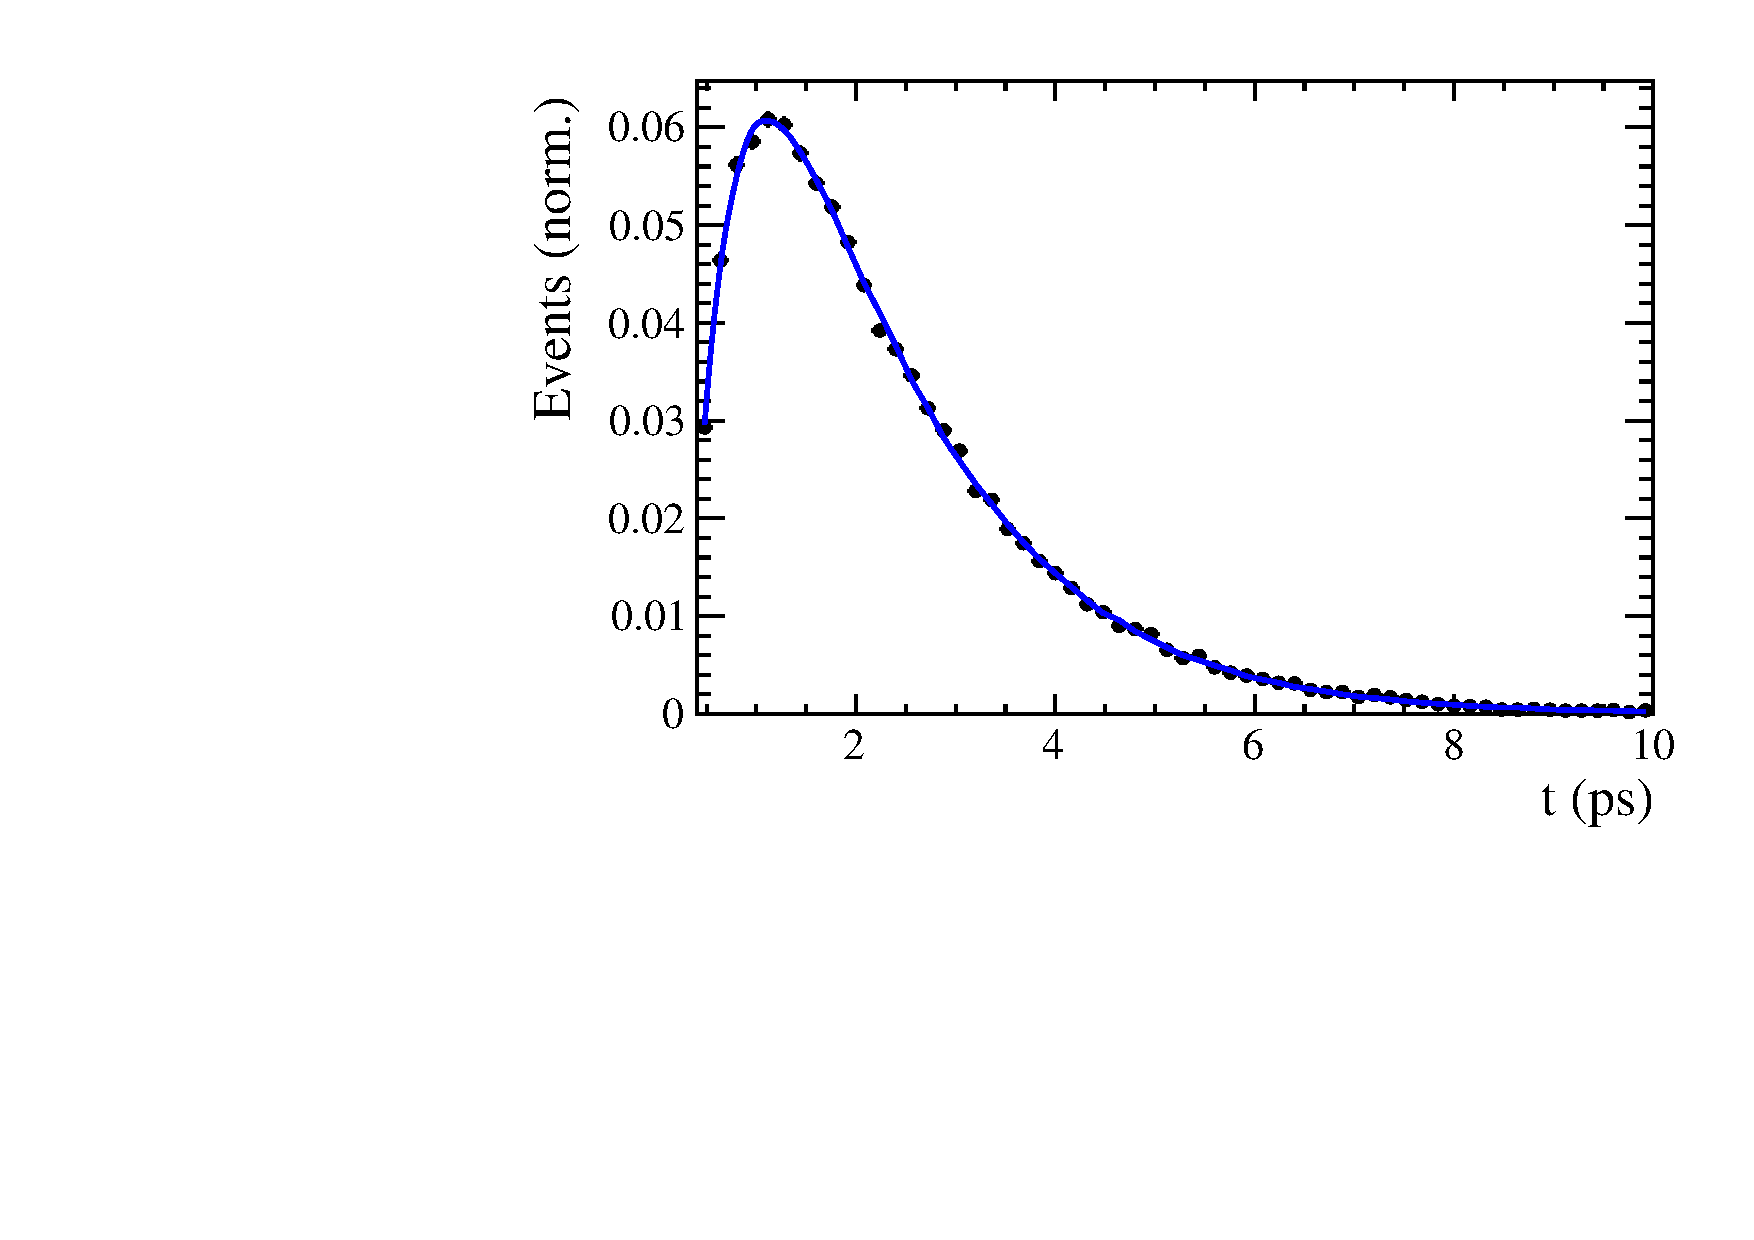
\includegraphics[width=0.4\textwidth, height = !]{figs/timeFit/norm_taggingCalib/h_t.pdf}
                %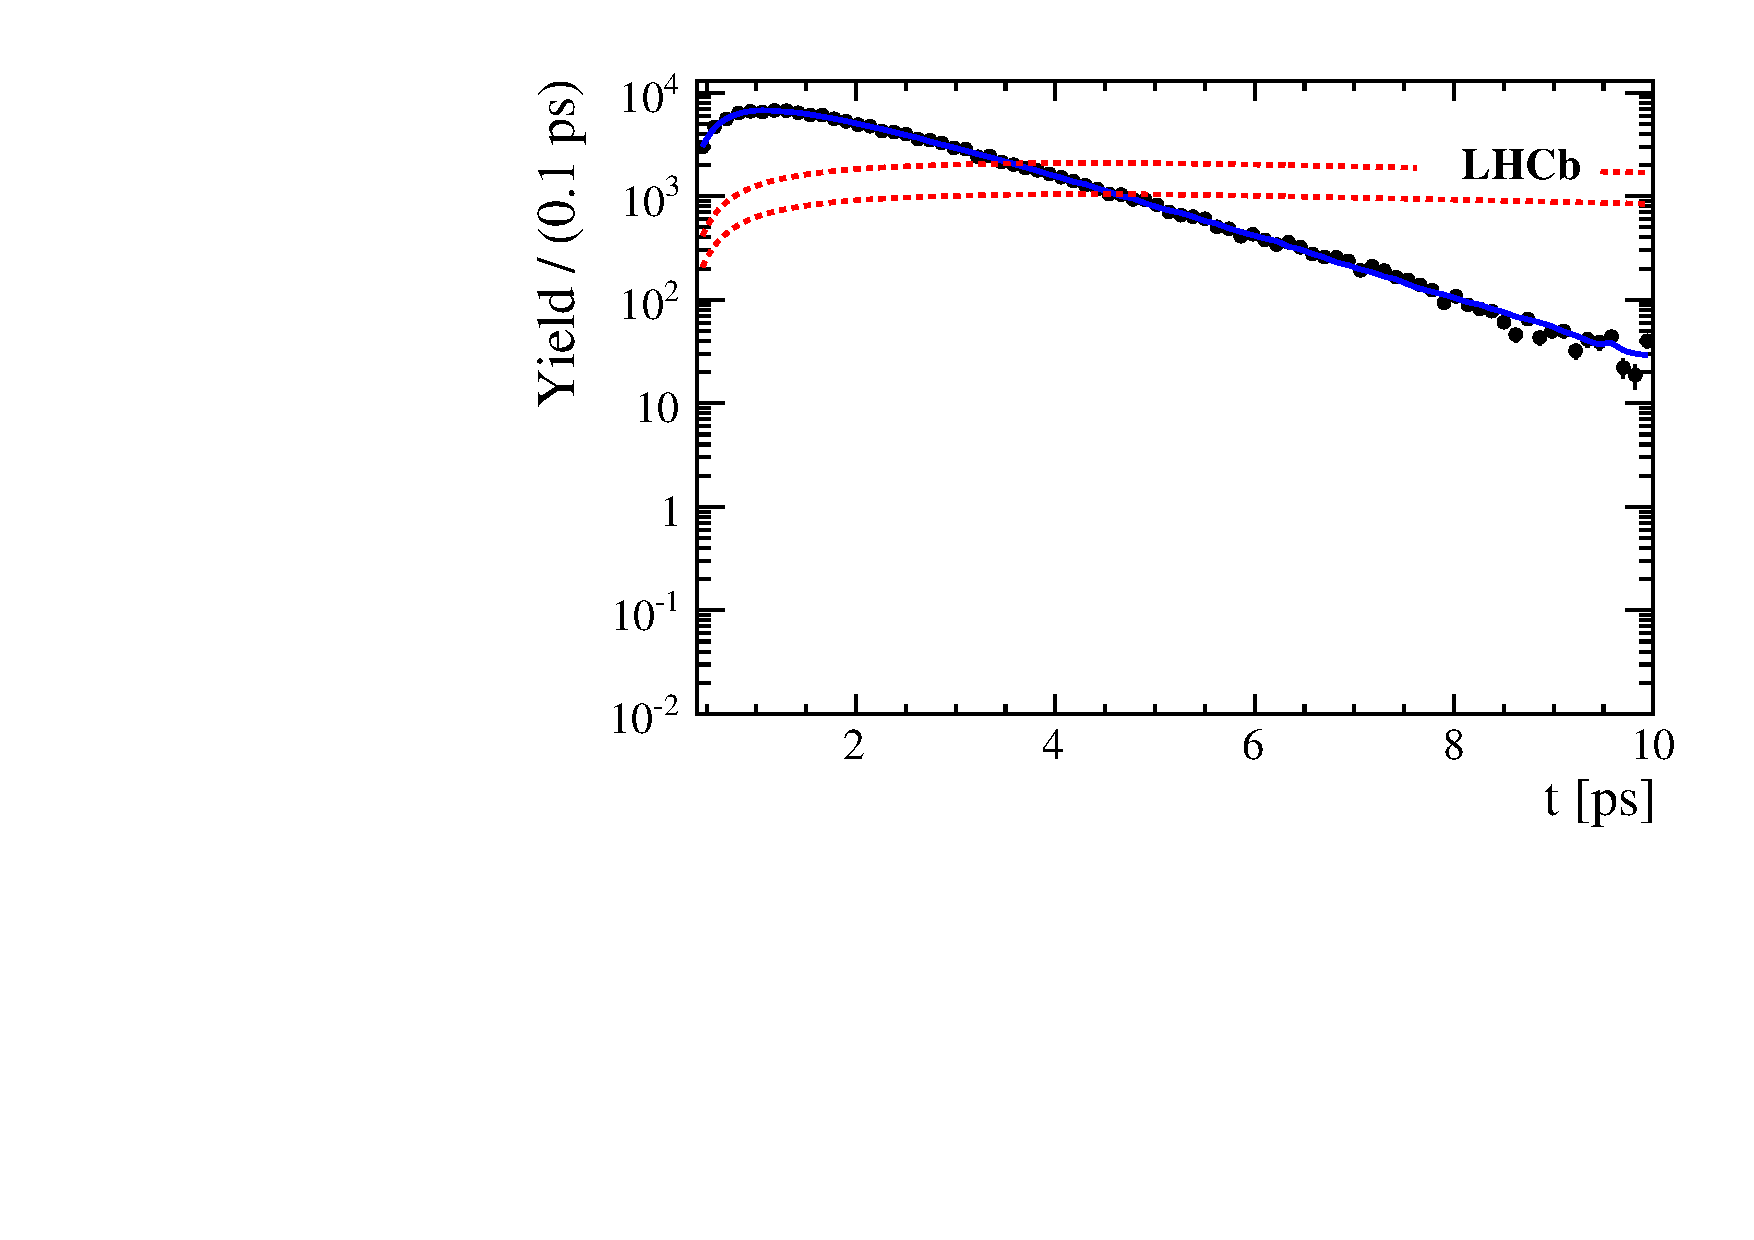
\includegraphics[width=0.4\textwidth, height = !]{figs/timeFit/norm_taggingCalib/h_t_log.pdf}
                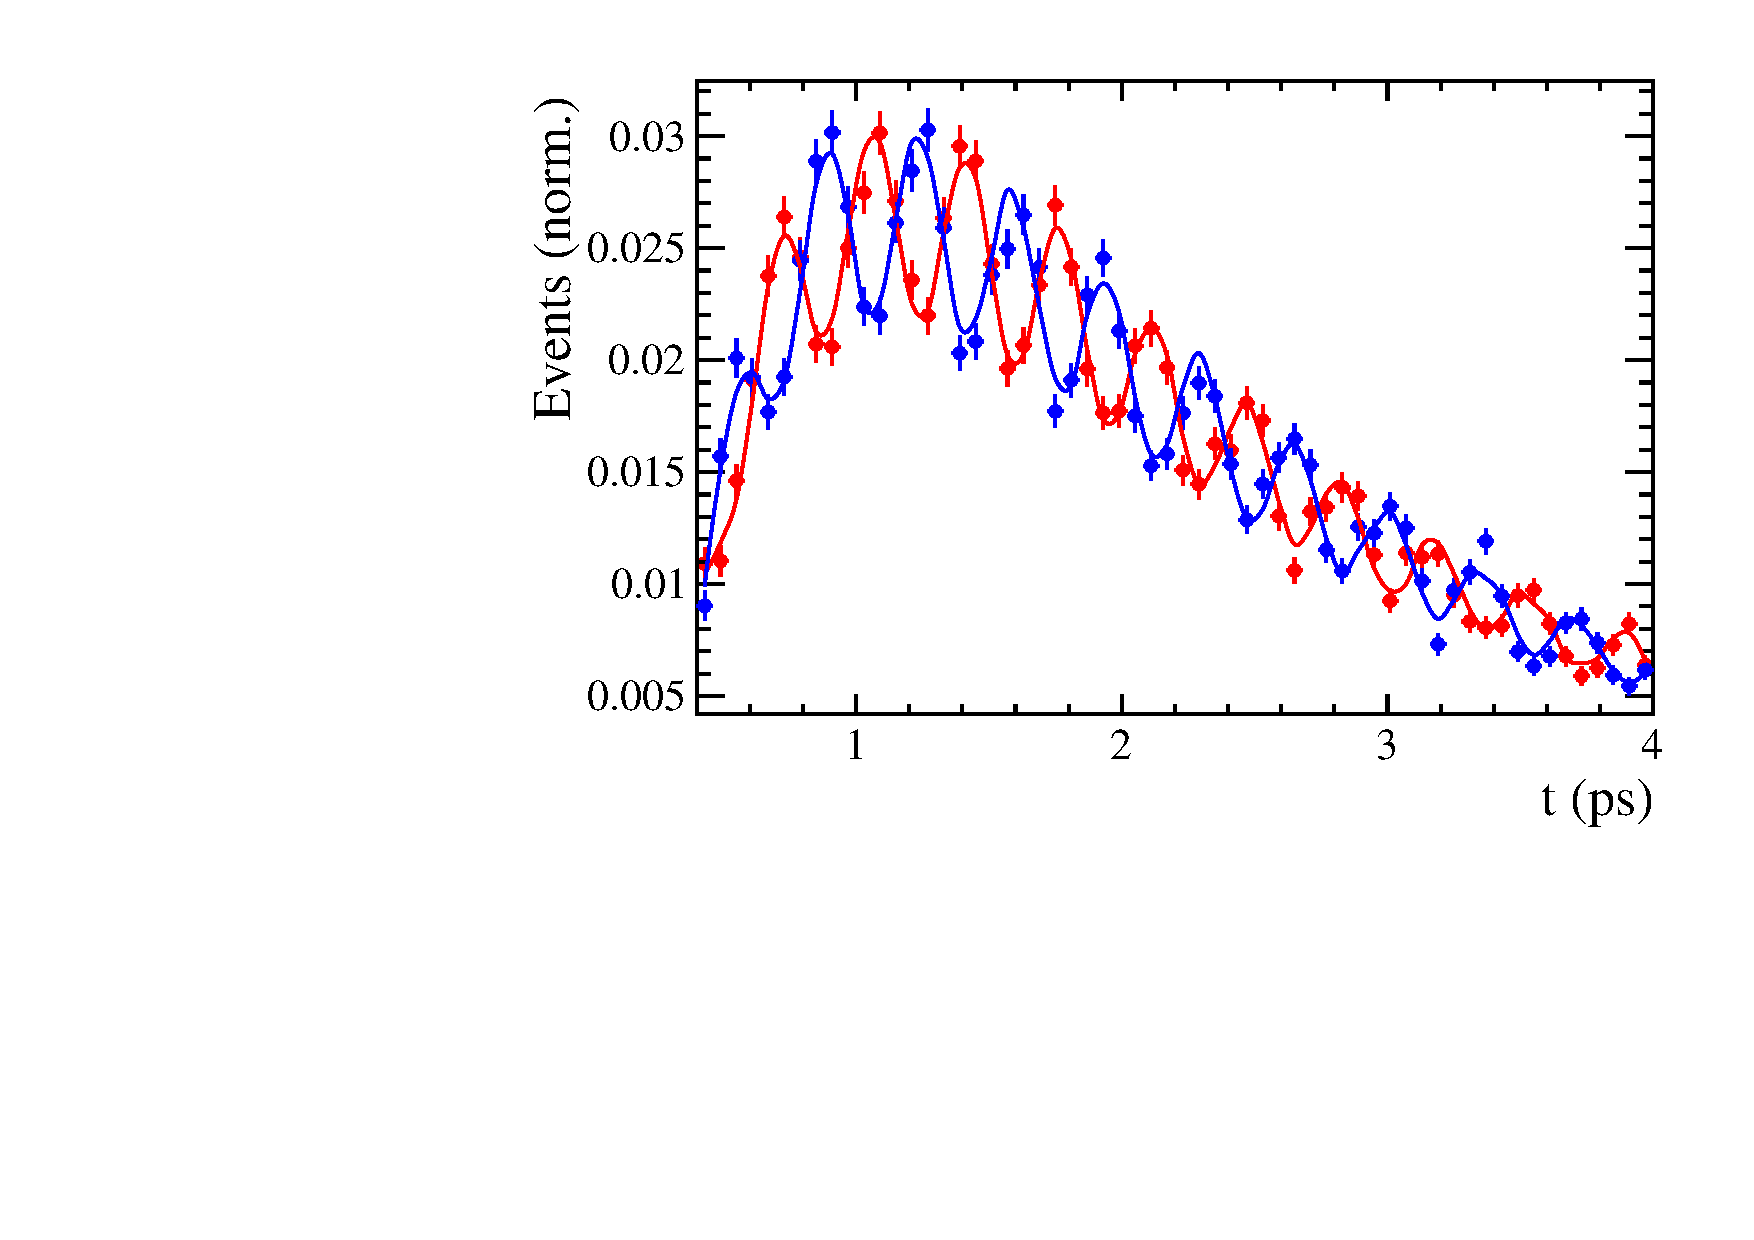
\includegraphics[width=0.4\textwidth, height = !]{figs/timeFit/norm_taggingCalib/h_t_mixed.pdf}
                %\includegraphics[width=0.4\textwidth, height = !]{figs/timeFit/norm_taggingCalib/h_asym.pdf}
                \caption{
Left: Flavour averaged decay-time distribution of $\Bs\to\Ds\pion\pion\pion$ candidates.
Right: Tagged decay-time distribution of mixed (red) and unmixed (blue) signal candidates.}
%Bottom-right: Time-dependent asymmetry $A_{mix}$ between mixed and unmixed $\Bs$ candidates folded into one oscillation period.}
                \label{fig:tFitNorm}
\end{figure}

The fit to $\Bs\to\Ds\kaon\pion\pion$ data is sensitive to a possible charge asymmetry of the kaon, introduced by its charge-dependent nuclear cross-section. 
Therefore, the detection asymmetry $A_{det}$ is introduced and multiplied as $(1 \pm A_{det})$, where the sign depends on the charge of the kaon, to the signal PDF. 
It is determined using a data-driven technique described in~\cite{Davis:2310213}.
The tagging calibration parameters are taken from the fit to the control sample and included in the fit using Gaussian-constrains.
The measured \CP coefficients are reported in Table \ref{tab:sigFitResults} and the fit projection is shown in Figure \ref{fig:tFitSig}.


\begin{table}[h]
\centering
\caption{\CP coefficients determined from a fit to the $B_s \to D_s K \pi\pi$ decay-time distribution. The uncertainties are statistical and systematic, respectively.}
%\resizebox{\linewidth}{!}{
        \renewcommand{\arraystretch}{1.5}
        \begin{tabular}{l c c c c } 
\hline
\hline
\multicolumn{1}{c}{Decay Channel} & \multicolumn{2}{c}{$A_{b \to c}$} & \multicolumn{2}{c}{$A_{b \to u}$}  \\ 
 & \multicolumn{1}{c}{$\vert a_i \vert$}  & \multicolumn{1}{c}{$arg(a_i) [\degrees]$}  & \multicolumn{1}{c}{$\vert a_i \vert$} & \multicolumn{1}{c}{$arg(a_i) [\degrees]$} \\ 
\hline
 $B_s \to D_s \, ( K_1(1270) \to K \, \rho(770) ) $ &  1.0 & 0.0 & 1.0 & 0.0  \\ 
$\phantom{B_s \to D_s \, (} K_1(1270) \to K^{*}(892) \, \pi \phantom{)} $ & 0.76 $\pm$ 0.11 $\pm$ 0.16 & 60.9 $\pm$ 9.6 $\pm$ 14.0 & &   \\ 
$\phantom{B_s \to D_s \, (} K_1(1270) \to K^{*}_{0}(1430) \, \pi \phantom{)} $ & 0.68 $\pm$ 0.06 $\pm$ 0.34 & 116.5 $\pm$ 5.1 $\pm$ 43.5 & &   \\ 
$B_s \to D_s \, ( K_1(1400) \to K^{*}(892) \, \pi ) $ & 2.53 $\pm$ 0.27 $\pm$ 0.57 & 12.9 $\pm$ 7.4 $\pm$ 8.0 & 0.67 $\pm$ 0.20 $\pm$ 0.51 & -76.3 $\pm$ 16.9 $\pm$ 22.8 \\ 
$B_s \to D_s \, ( K^{*}(1410) \to K^{*}(892) \, \pi ) $ & 1.28 $\pm$ 0.12 $\pm$ 0.24 & 54.9 $\pm$ 5.6 $\pm$ 9.8 &  &  \\ 
$\phantom{B_s \to D_s \, (} K^{*}(1410) \to K \, \rho(770) \phantom{)} $ & 0.66 $\pm$ 0.04 $\pm$ 0.03 & -172.9 $\pm$ 5.0 $\pm$ 6.5 & &   \\ 
$B_s \to D_s \, ( K(1460) \to K^{*}(892) \, \pi ) $ & & &0.77 $\pm$ 0.11 $\pm$ 0.62 & -93.6 $\pm$ 11.2 $\pm$ 12.1 \\ 
$B_s \to ( D_s \, \pi)_{P} \, \, K^{*}(892) $ & 1.02 $\pm$ 0.13 $\pm$ 0.41 & -28.4 $\pm$ 8.0 $\pm$ 10.4 & 0.79 $\pm$ 0.18 $\pm$ 0.35 & 3.7 $\pm$ 12.5 $\pm$ 14.8 \\ 
$B_s \to ( D_s \, K)_{P} \, \, \rho(770) $ & & &0.61 $\pm$ 0.08 $\pm$ 0.26 & 36.4 $\pm$ 7.7 $\pm$ 14.1 \\ 
\hline
\hline
\multicolumn{1}{c}{Fit parameter} & \multicolumn{4}{c}{Value}  \\ 
\hline
\multicolumn{1}{c}{$m_{K_1(1400)} \, [\text{MeV}]$} & \multicolumn{4}{c}{1394.9 $\pm$ 8.8 $\pm$ 12.6 $\pm$ 21.2} \\ 
\multicolumn{1}{c}{$\Gamma_{K_1(1400)} \, [\text{MeV}]$} & \multicolumn{4}{c}{224.0 $\pm$ 15.9 $\pm$ 22.0 $\pm$ 20.9} \\ 
\multicolumn{1}{c}{$m_{K^{*}(1410)} \, [\text{MeV}]$} & \multicolumn{4}{c}{1419.6 $\pm$ 10.8 $\pm$ 26.8 $\pm$ 24.1} \\ 
\multicolumn{1}{c}{$\Gamma_{K^{*}(1410)} \, [\text{MeV}]$} & \multicolumn{4}{c}{342.4 $\pm$ 23.5 $\pm$ 51.0 $\pm$ 52.9} \\ 
 \\ 
\multicolumn{1}{c}{$r$} & \multicolumn{4}{c}{xx.xx $\pm$ 0.04 $\pm$ 0.05 $\pm$ 0.04} \\ 
\multicolumn{1}{c}{$\delta \, [\degrees]$} & \multicolumn{4}{c}{xx.xx $\pm$ 16.1 $\pm$ 6.2 $\pm$ 6.8} \\ 
\multicolumn{1}{c}{$\gamma - 2 \beta_{s} \, [\degrees]$} & \multicolumn{4}{c}{xx.xx $\pm$ 16.1 $\pm$ 11.4 $\pm$ 6.2} \\ 
\hline
\hline
\end{tabular}

%}
\label{tab:sigFitResults}
\end{table}

\begin{figure}[h]
        \centering
                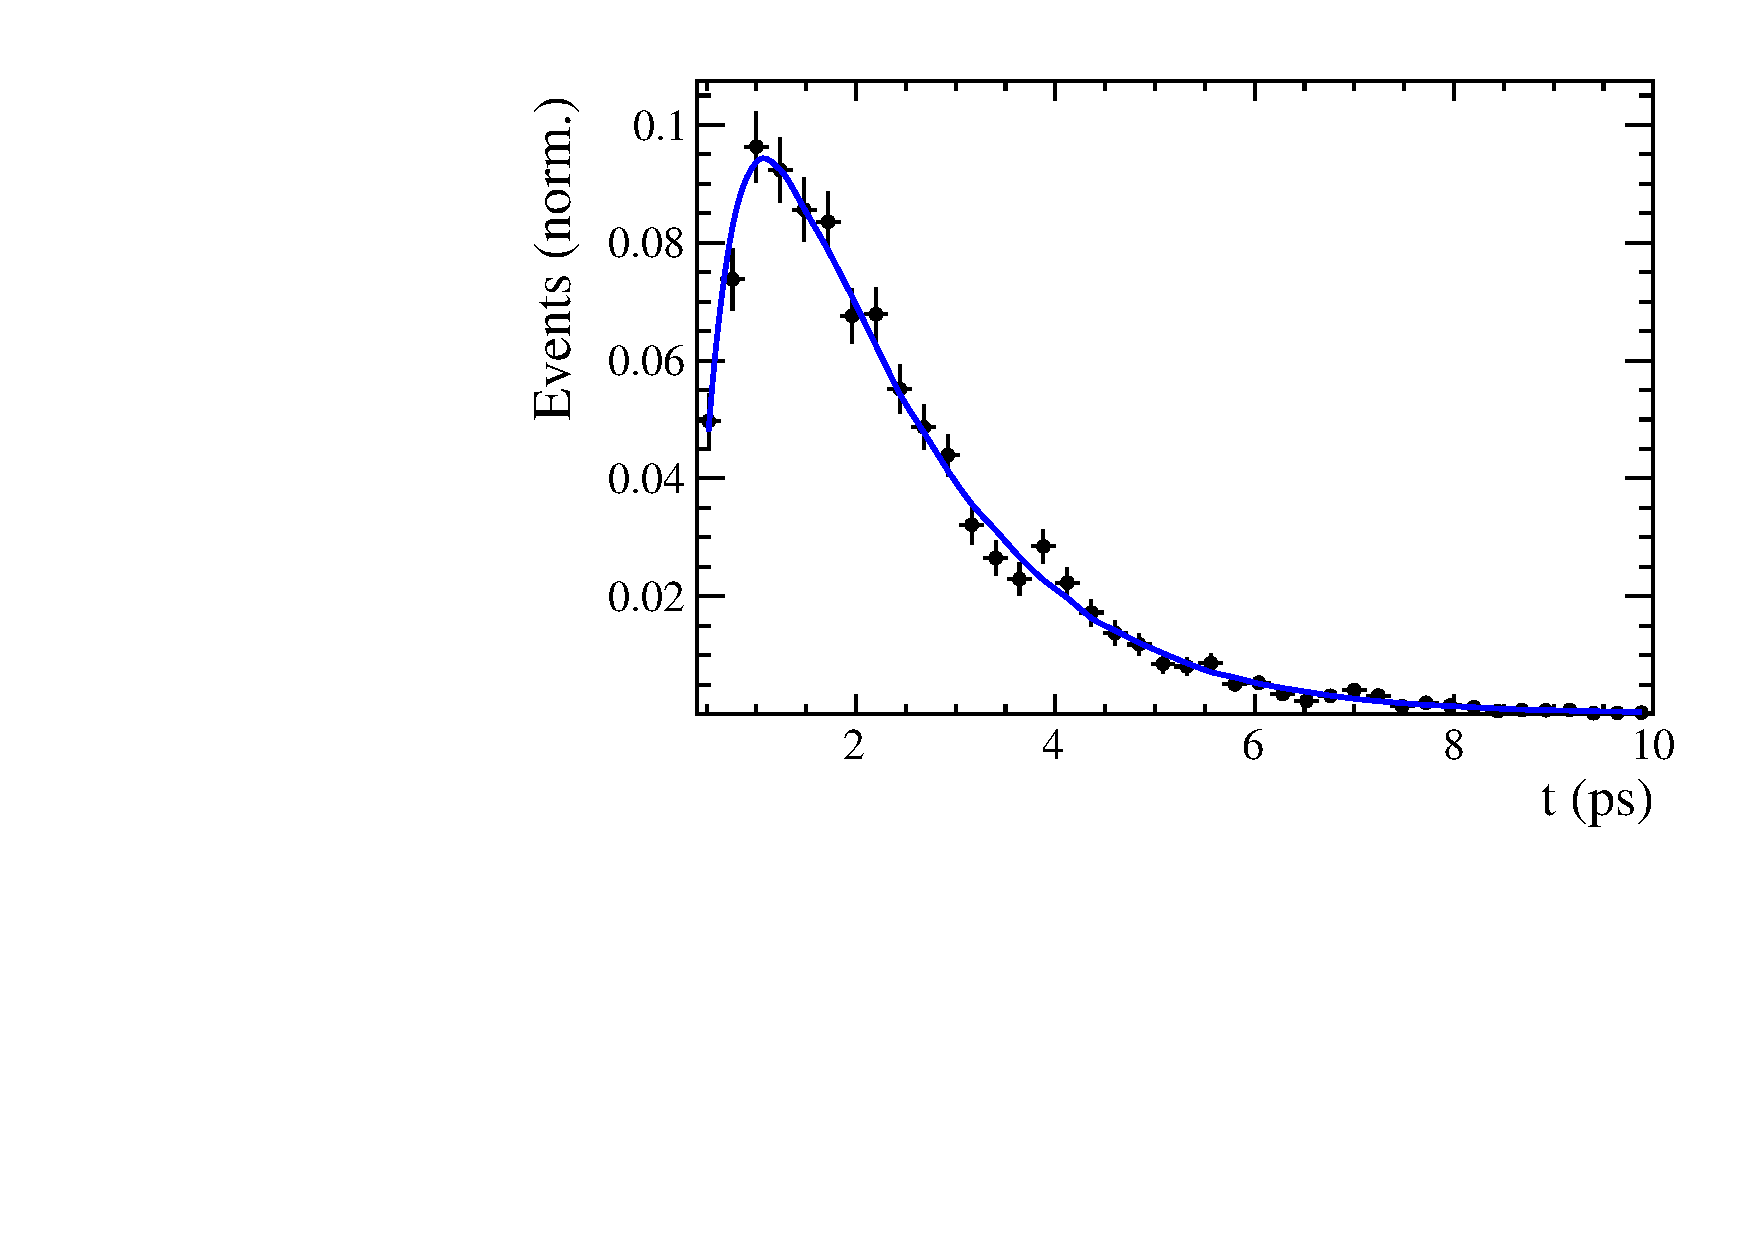
\includegraphics[width=0.4\textwidth, height = !]{figs/timeFit/signal/h_t.pdf}
                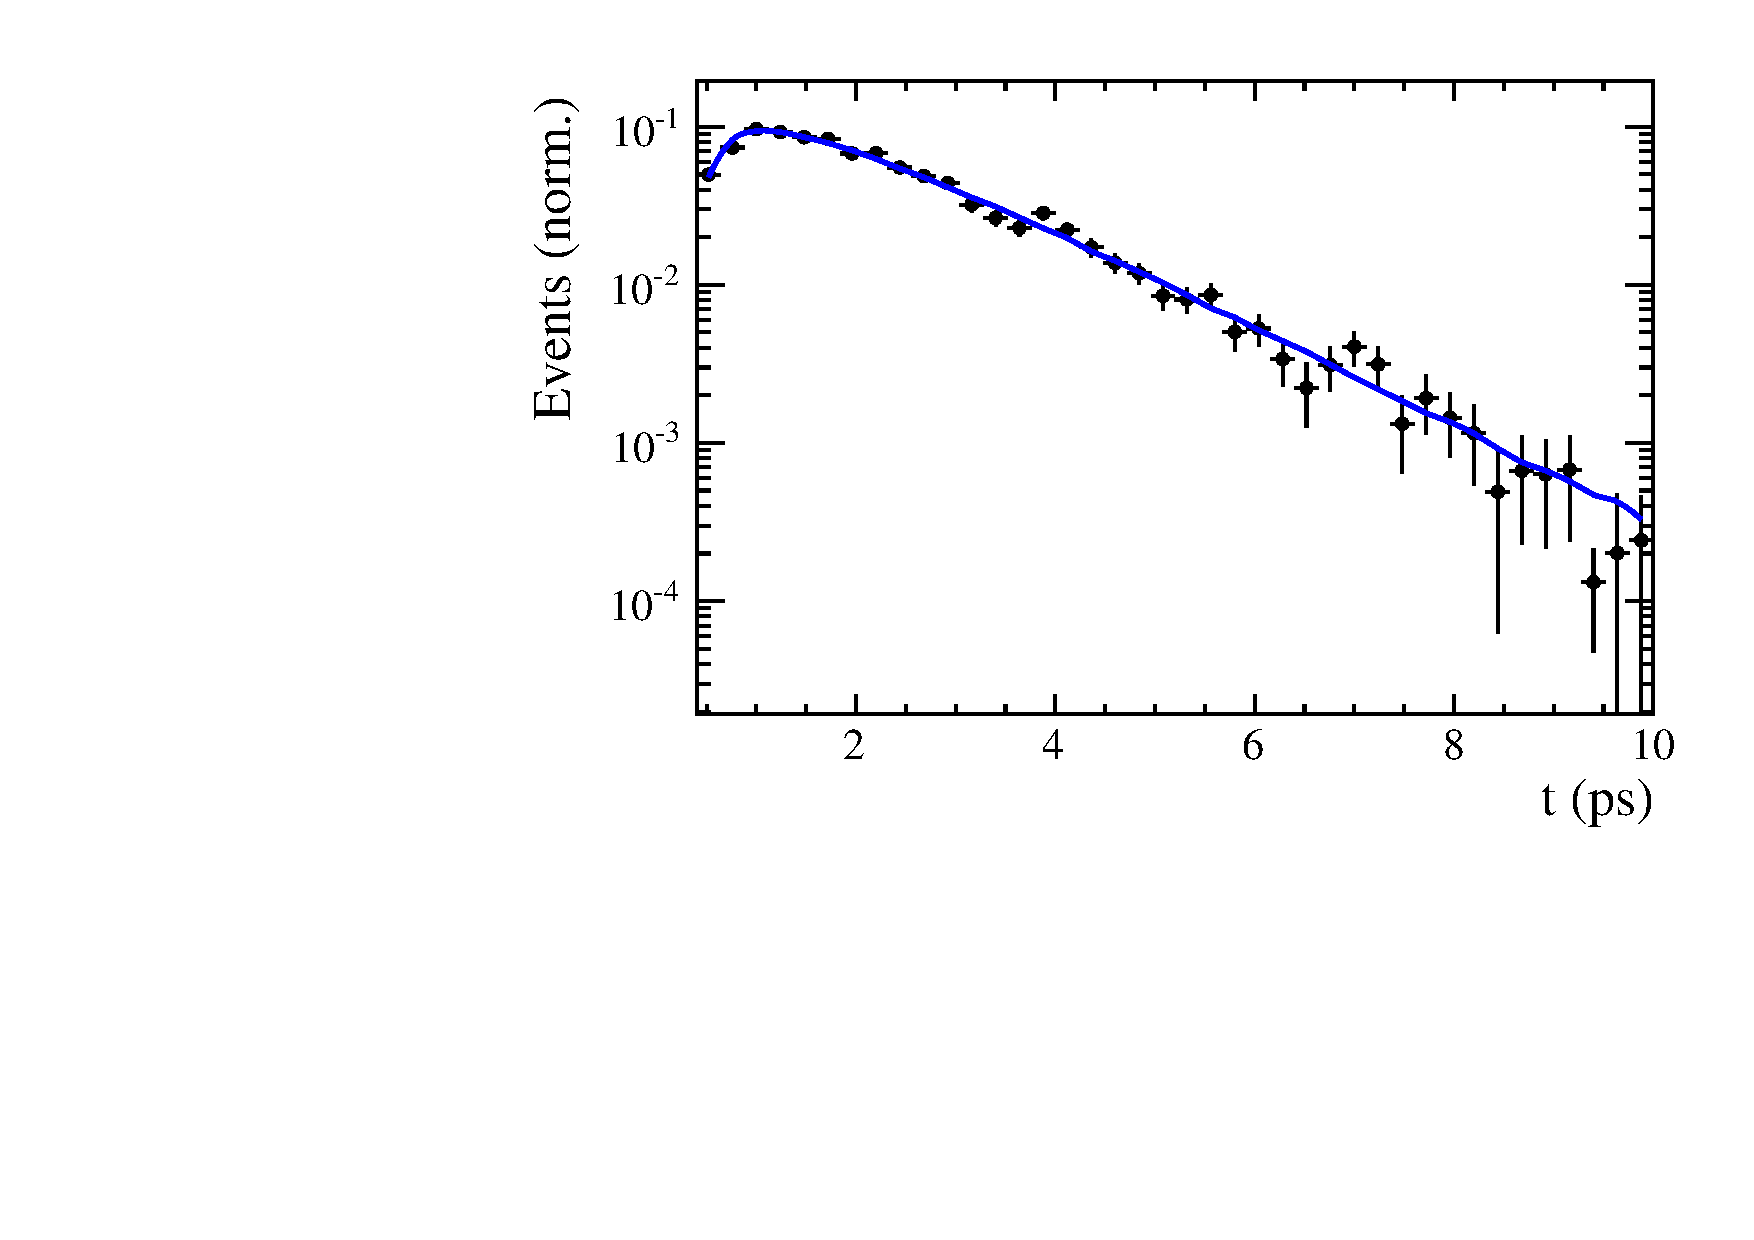
\includegraphics[width=0.4\textwidth, height = !]{figs/timeFit/signal/h_t_log.pdf}
%               \includegraphics[width=0.45\textwidth, height = !]{figs/timeFit/signal/h_asym.pdf}              
                \caption{Decay-time distribution of $\Bs\to\Ds\kaon\pion\pion$ signal candidates with the fit projection overlaid in (left) regular and (right) logarithmic scale.}
                \label{fig:tFitSig}
\end{figure}
